\section{DF model dynamics} 
% FOR ALL FORCES: 
    % define them 
    % explain how they get computed 
% Show a simulation run with all forces combined 
% also explained the numerical solver and method that gets used 
We characterise the interaction force $\F$ as the sum of gradient flows of energies. \\
% TODO: Change desired state before minus in each force !!!
A gradient flow describes how a system changes over time in a way that always reduces a given energy $E(\vec{C})$.
To obtain the gradient flow of this energy on vertex $\vec{v}$, we must add the term $-\nabla_{\vec{v}} E(\vec{C})$ to $\F$.
Since all our energy terms are positive, the lowest possible value is zero.  
So, the gradient flow moves the system step by step toward this minimum, always trying to decrease the energy until, ideally, it reaches zero. 
This is how we guide the motion of our cells: by letting them follow the gradient flow of each energy so that their shapes and vertex positions gradually adjust to reduce the total energy. \\
In~\cite{Vogel2023}, the area, edge, interior angle, and overlap energies were introduced.
The first three energies are responsible for maintaining the shape of each cell. 
All of these three according forces act on each cell in a vacuum based only on its own current cell shape. \\
Unlike in~\cite{Vogel2023}, where each cell was assigned an individual desired state, we now assume a common desired state for all cells. This simplification allows for a more controlled analysis of the system's deformability and its influence on the collective dynamics.
We assume that all cells are initially given in their desired states in order to prevent system instabilities right from the beginning. \\
Additionally, we introduce slight modifications to the energy formulation: rather than being defined locally on vertices or edges, the energies are now defined over entire cells. 
This adjustment provides a more coherent basis for deriving cell-level forces and ensures consistency with the global dynamic framework introduced in this study. \\
Interactions between different cells just arise from the overlap force, which acts to resolve overlaps and to prevent cell interpenetration. 
In the process of resolving overlaps, the shape of the cells will change.  
Once the overlap is resolved, the first three forces act to restore the cell's original shape. \\
The central question we aim to investigate in this thesis is how the deformability of individual cells influences the overall diffusivity of the cell system.
But first, let us introduce each of the mentioned forces. \\
We define our energies as
\[E_k(x) = \frac{1}{k} |x_{\text{desired}} - x_{\text{current}}|^k, \]
where $k \in \N_{\geq 1}$ is a positive integer parameter specific to each energy term. 
Using different values of $k$ allows us to model various types of energies and their corresponding forces, resulting in distinct dynamical behaviors that reflect different aspects of cell physics. \\
In order to compute the forces arising from these energy functions, we require the gradient $\nabla E$. 
This leads us to compute derivatives of the form 
\[ \frac{\dequ}{\dequ x} |x|^k. \]
While $|x|^k$ is not classically differentiable at $x=0$, it is weakly differentiable for all $k \in \N_{\geq 1}$.
There exists a locally integrable function 
\[ x \mapsto k \sgn(x)|x|^{k-1} \in L^1_{loc}(\R),\] 
such that for all $\phi \in C_C^{\infty}(\R)$:
\begin{align*}
	\int_{\R} |x|^k \phi'(x) \dequ x  
	&= \int_{\R_{\geq 0}} x^k \phi'(x) \dequ x + \int_{\R_{< 0}} (-x)^k \phi'(x) \dequ x \\
	&= [x^k \phi(x)]_{0}^{\infty} - \int_{\R_{\geq 0}} k x^{k-1} \phi(x) \dequ x + [(-x)^k \phi(x)]_{0}^{\infty} - \int_{\R_{< 0}} k (-x)^{k-1} \phi(x) \dequ x \\
	&= - \int_{\R_{\geq 0}} k x^{k-1} \phi(x) \dequ x - \int_{\R_{< 0}} k (-x)^{k-1} \phi(x) \dequ x \\
	&= - \int_{\R} k \sgn(x)|x|^{k-1} \phi(x) \dequ x.
\end{align*}
Thus, $x \mapsto k \sgn(x)|x|^{k-1}$ is the weak derivative of $x \mapsto |x|^k$. 
We will use this weak derivative for all of our force computations. 

\subsection{Area force}
The area force is designed to maintain each cell's area close to a preferred target value. 
In order to compute a cells area, which is the area of a positively orientated polygon, we can use the Shoelace formula from~\cite{Shoelace2014}. 

\begin{proposition}  \textbf{Shoelace formula for DF cells} \label{prop:Shoelace}\\ 
	Let $C = (\vec{v}_1, \ldots, \vec{v}_N)$ be a DF cell with $\vec{v}_j = (v_j^{x}, v_j^{y})^T$ for $j=1,\ldots,N$.
	We determine the area $A_C$ of $C$ by applying the Shoelace formula
	\begin{center}
		$A_C = \frac{1}{2}\sum\limits_{j = 1}^{N} (v_j^{x} v_{j+1}^{y} - v_{j+1}^{x} v_j^{y})$,
	\end{center} 
	where $\vec{v}_{N + 1} = \vec{v}_1$. \\
	Proof. 	\\
	An illustration supporting the proof is provided in \ref{fig:shoelace}, which is where the idea of the proof comes from. 
	Without loss of generality, we may assume that all coordinates are positive.
	If this is not initially the case, the entire polygon can be translated into the positive quadrant without affecting its area. \\
	For each $1 \leq j \leq N$ the edge $\overline{ \vec{v}_j \: \vec{v}_{j+1}}$ is associated with the area $T_j$ of the trapeze that arises when connecting the line segment vertically with the $x$ axis. 
	The signed trapeze area of $T_j$ can be computed with 
	\begin{center}
		$T_j = \frac{1}{2} (v_j^{y} + v_{j+1}^{y})(v_j^{x} - v_{j+1}^{x})$.
	\end{center}
	The area $T_j$ has a positive sign if $v_j^{x} \geq v_{j+1}^{x}$ (green arrow in Figure \ref{fig:shoelace}) and a negative sign otherwise (red arrow). 
	As depicted in the figure, the negatively signed areas precisely cancel the excess portions that would result from summing only the positively signed trapezoids.
	Thus the total polygon's area is equal to the sum of all trapezes
	\begin{center}
		$A_C = \sum\limits_{j = 1}^{N} T_j = \frac{1}{2} \sum\limits_{j = 1}^{N} (v_j^{y} + v_{j+1}^{y})(v_j^{x} - v_{j+1}^{x}) = \frac{1}{2}\sum\limits_{j = 1}^{N} (v_j^{x} v_{j+1}^{y} - v_{j+1}^{x} v_j^{y}) $.
	\end{center} 
	\begin{figure}
		\begin{center}
			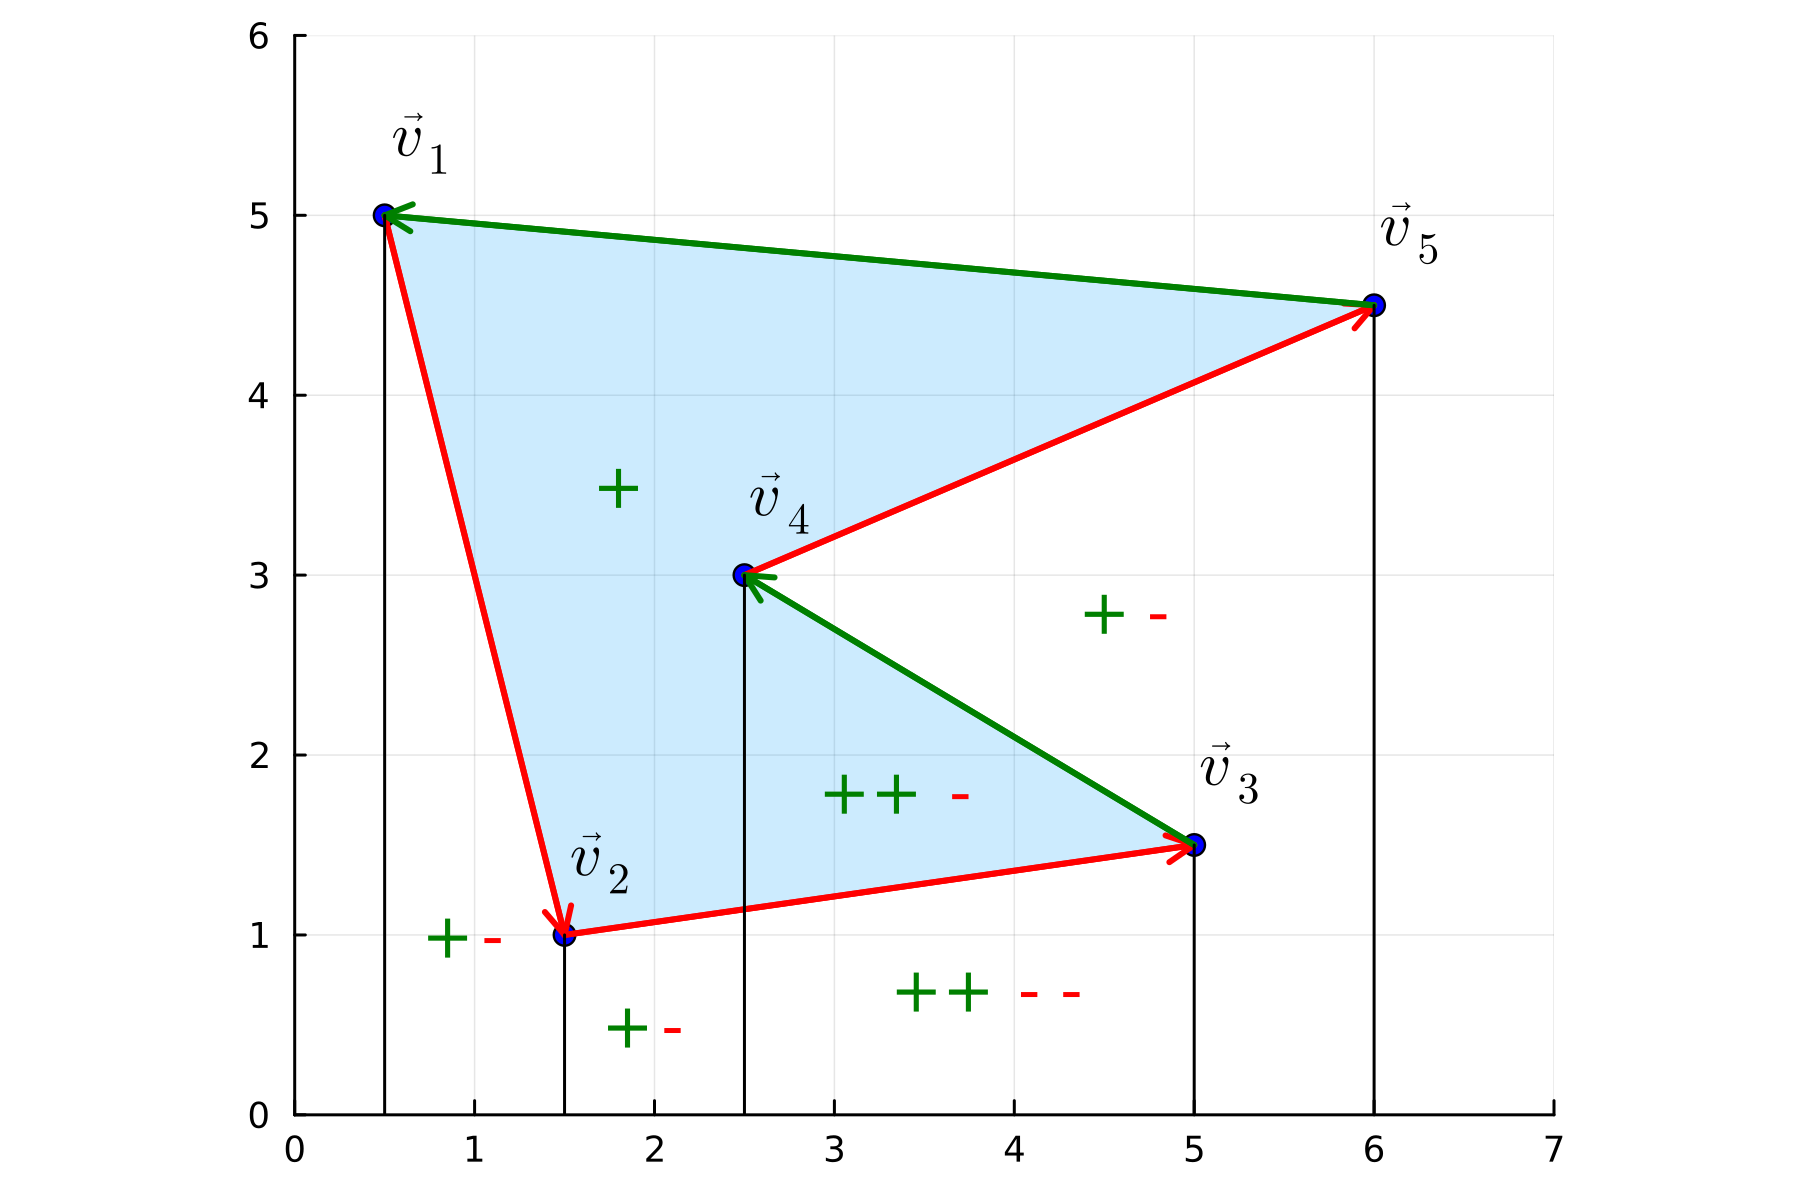
\includegraphics[width=8cm]{bachelors-thesis/shoelace_new.png}
			\caption{
				This figure shows a geometrical interpretation of the shoelace formula.
				The green arrows, which point from right to left, represent positive trapezoidal areas that contribute positively to the total area of the polygon.
				In contrast, the red arrows point from left to right and represent negative areas that are subtracted in the computation.
				The vertical black lines divide the plot into subregions.
				Within each subregion, green arrows are counted with plus signs and red arrows with minus signs.
				We observe that the subregions lying outside the polygon contain an equal number of plus and minus signs, indicating that their net contribution to the area is zero.
				In contrast, the subregions inside the polygon always have one more plus sign than minus signs, meaning their area is counted exactly once in the total.
				Overall, this illustrates that the method correctly computes the area of the polygon.
				Source:~\cite{ShoelaceFigure2022}}
			\label{fig:shoelace}
		\end{center}
	\end{figure}
	\qed
\end{proposition}

With the Shoelace formula we are able to easily compute all cell areas at all times in the simulation. 
This enables us to implement the gradient flow over the area energy. 

\begin{definition} \textbf{Area energy} \\
The energy $A_k: (\R^2)^{N_V} \rightarrow \R_{\geq 0}$ for $k \in \N_{\geq 1}$, used to keep the cells at a constant volume, reads 
	\begin{align}
		A_k(C) = \frac{1}{k} |A_{C} - A_d|^k, \label{eq:areaEnergy} 
	\end{align}
	where $A_d$ is the desired cell area of all cells and $A_{C}$ is the current area of cell $i$. 
\end{definition}

To maintain the cell area during the simulation, we evaluate the gradient flow of the area energy which indicates the direction of motion for each vertex for preserving the cell area.

\begin{proposition} \textbf{Area force} \label{force:area}\\
	The area force $F_{k}^{(A)}: (\R^2)^{N_V} \rightarrow (\R^2)^{N_V}$ that gets applied on cell $C$ is given by  
	\begin{align*}
		F_{k}^{(A)}(C) 
		= - (\nabla_{\vec{v}_1} A_k(C), \ldots, \nabla_{\vec{v}_{N_V}} A_k(C))^T,
	\end{align*}
	where the gradient $\nabla_{\vec{v}_j} A_k(C)$ with respect to $\vec{v}_j = (v_{j}^{x}, v_{j}^{y})^T$ is given by 
	\begin{align}
		\nabla_{\vec{v}_j} A_k(C) = \dfrac{1}{2} \sgn(A_{C} - A_d) |A_{C} - A_d|^{k-1} \begin{pmatrix} v_{j+1}^{y} - v_{j-1}^{y} \\[0.5em]  v_{j-1}^{x} - v_{j+1}^{x} \end{pmatrix},
		\label{gradient:area}
	\end{align}
	for all $1 \leq j \leq N_V$.\\


	Proof.\\
	Choose $1 \leq j \leq N_V$.  
 
	\begin{align*}
		\nabla_{\vec{v}_j} A_k(C) &= \frac{1}{k} \nabla_{\vec{v}_j} | A_{C} - A_d |^k  \\ 
		&= \sgn(A_{C} - A_d) | A_{C} - A_d |^{k-1} \nabla_{\vec{v}_j} (A_{C} - A_d) \\
		&= \sgn(A_{C} - A_d) | A_{C} - A_d |^{k-1} \nabla_{\vec{v}_j} A_{C} \\
		&= \sgn(A_{C} - A_d) | A_{C} - A_d |^{k-1} \nabla_{\vec{v}_j} (\frac{1}{2} \sum\limits_{k = 1}^{N} (v_k^{x} v_{k+1}^{y} - v_{k+1}^{x} v_k^{y})) \\[0.5em]  
		&= \frac{1}{2} \sgn(A_{C} - A_d) | A_{C} - A_d |^{k-1} \begin{pmatrix}
				\partial_{v_j^{x}} (v_j^{x} v_{j+1}^{y} - v_j^{x} v_{j-1}^{y})  \\[0.5em]
				\partial_{v_j^{y}} (v_{j-1}^{x} v_j^{y} - v_{j+1}^{x} v_j^{y})
			\end{pmatrix} \\[0.5em] 
		&= \frac{1}{2} \sgn(A_{C} - A_d) | A_{C} - A_d |^{k-1} \begin{pmatrix}
				v_{j+1}^{y} - v_{j-1}^{y}  \\
				v_{j-1}^{x}  - v_{j+1}^{x} 
			\end{pmatrix} 
	\end{align*}

	Remember that $A_d$ is just an independent constant. 
	\qed
\end{proposition}
It is also valid to write $F_{j}^{(A)}(\vec{C})$ instead of $F_{j}^{(A)}(C)$, since $C$ is included in $\vec{C}$. 


\begin{figure}
	\begin{center}
		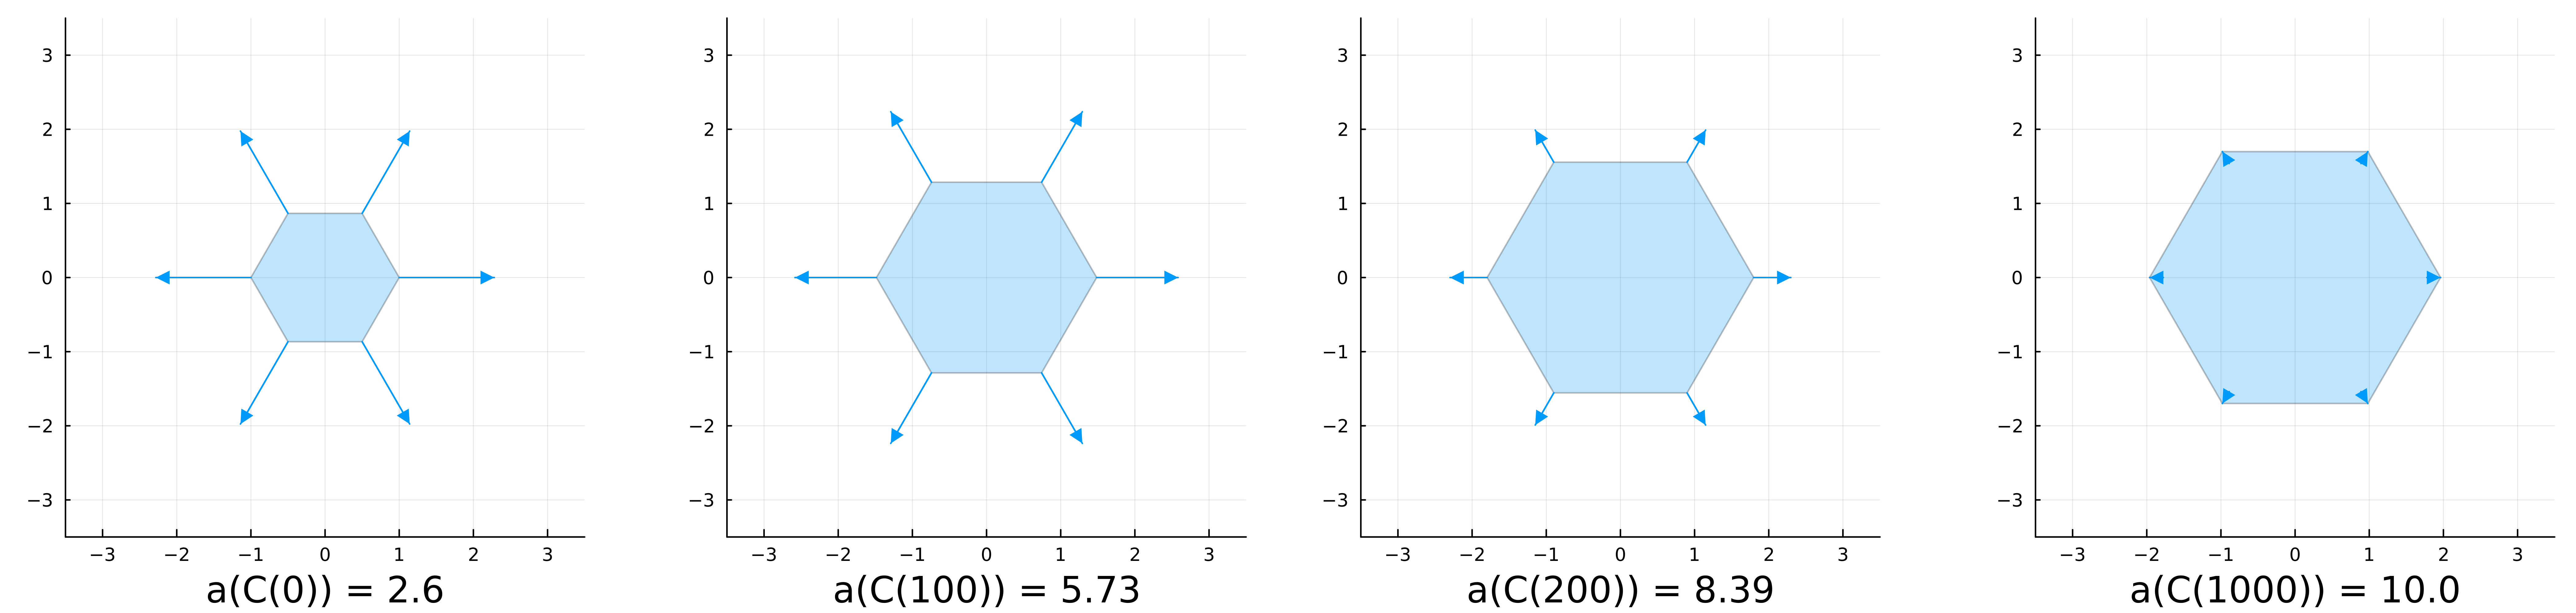
\includegraphics[width=15cm]{bachelors-thesis/forces/area1/area1.png}
		\caption{The figure displays the solution of Model  
		Initially, the cell has an area of approximately $2.6$. 
		Arrows originating from each vertex represent the forces acting on the vertices at the corresponding time.
		The area force acts by pushing the vertices outward from the cell center, resulting in an increase in area.
		The computed areas at each time step are indicated below the respective diagrams.
		We can observe that the forces decrease as the actual cell area gets closer to its desired state. 
		Once the target area of $A_d = 10.0$ is reached, the force vanishes and the system reaches a steady state.
		}
		\label{fig:areaForce}
	\end{center}
\end{figure}

\begin{figure}
	\begin{center}
		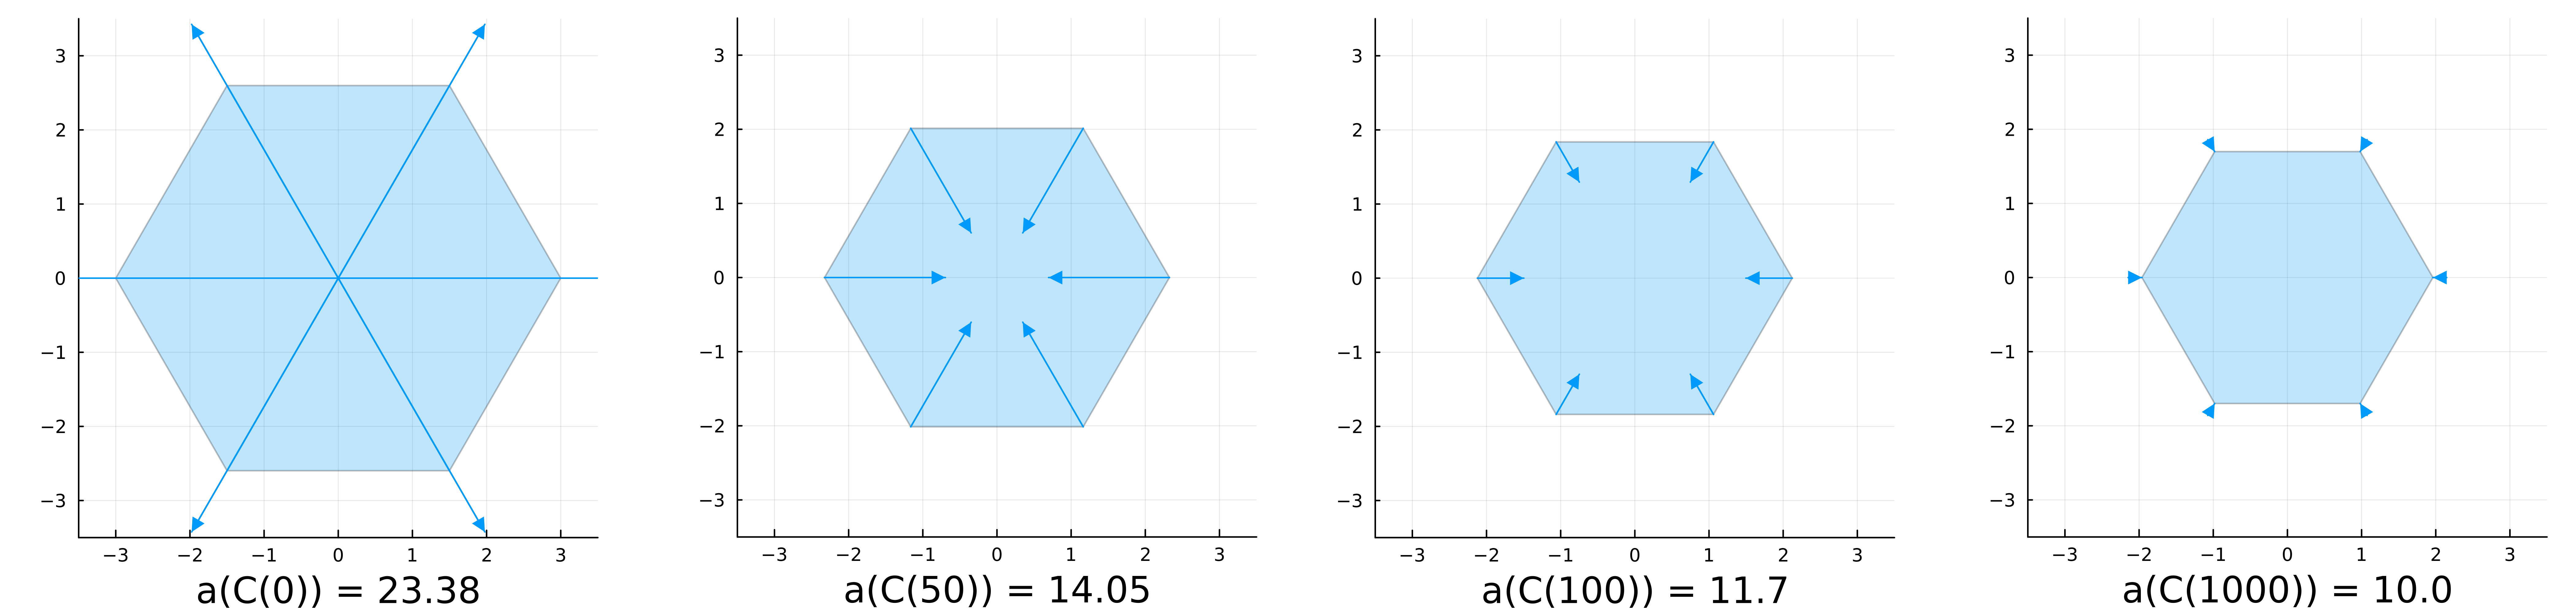
\includegraphics[width=15cm]{bachelors-thesis/forces/area2/area2.png}
		\caption{Similar to Figure \ref{fig:areaForce}, this image shows a cell that develops according to the area force. 
		In contrast to the previous illustration, the initial area is now larger than the desired target area.
		As a result, the area force needs to reverse its direction to shrink the cell toward the target area $A_d = 10.0$
		This outcome is consistently demonstrated across the four diagrams. }
		\label{fig:areaForce2}
	\end{center}
\end{figure}

Figures \ref{fig:areaForce} and \ref{fig:areaForce2} illustrate how the area force acts on a cell to either expand or contract it toward the desired target area.

    
\subsection{Edge force}
The next force we would like to model is the edge force. 
It acts on the cells' edges and aims to maintain their lengths.
We define the edge $1 \leq j \leq N_V$ as 
\begin{center}
	$
	e_j = \overline{\vec{v}_j \: \vec{v}_{j+1}}
	$
\end{center}
and we use the operator 
\begin{center}
	$
	E^j_C = \norm[\vec{v}_j - \vec{v}_{j+1}]
	$
\end{center}
to compute the length of the edge. 

The according energy for this edge is:
\begin{definition} \textbf{Edge energy} \\
	The energy $E_k: (\R^2)^{N_V} \rightarrow \R_{\geq 0}$, used to keep the edges at a constant length, reads 
	\begin{align}
		E_k(C) =  \sum\limits_{j=1}^{N_V} \frac{1}{k} |E^j_{C} - E^{j}_d|^k, \label{eq:edgeEnergy} 
	\end{align}
	where $E^j_{C}$ is the current edge length and $E^{j}_d$ is the desired edge length of edge $j$. 
\end{definition}

Since each vertex $\vec{v}_j$ influences exactly the edge lengths of the edges $e_{j}$ and $e_{j-1}$, we get the total edge force on $\vec{v}_j$ with: 

\begin{proposition} \textbf{Edge force} \\

	The edge force $F_{k}^{(E)}: (\R^2)^{N_V} \rightarrow (\R^2)^{N_V}$ that gets applied on cell $C$ is given by  
	\begin{align*}
		F_{k}^{(E)}(C) 
		= - (\nabla_{\vec{v}_1} E_k(C), \ldots, \nabla_{\vec{v}_{N_V}} E_k(C))^T,
	\end{align*}
	where the gradient $\nabla_{\vec{v}_j} E_k(C)$ with respect to $\vec{v}_j = (v_{j}^{x}, v_{j}^{y})^T$ is given by 
	\begin{align}
		\begin{split}
			\nabla_{\vec{v}_j} E_k(C) &= \sgn(E^{j-1}_{C}- E_d^{j-1}) \dfrac{|E^{j-1}_{C}- E_d^{j-1}|^{k-1}}{E^{j-1}_{C}}  
			\begin{pmatrix} v_{j}^{x} - v_{j-1}^{x} \\[0.5em]  v_{j}^{y} - v_{j-1}^{y}  \end{pmatrix} \\[0.5em]
			&+ \sgn(E^j_{C} - E_d^{j}) \dfrac{|E^j_{C} - E_d^{j}|^{k-1}}{E^j_{C}}  
			\begin{pmatrix} v_{j}^{x} - v_{j+1}^{x} \\[0.5em]  v_{j}^{y} - v_{j+1}^{y} \end{pmatrix}
		\end{split}
		\label{gradient:edge}
	\end{align}
	for all $1 \leq j \leq N_V$.\\

	Proof. \\

	\begin{align*}
		\nabla_{\vec{v}_{j}} E(C) &= \nabla_{\vec{v}_{j}} \sum\limits_{j=1}^{N_V} \frac{1}{k} |E^j_{C} - E^{j}_d|^k \\
		&= \frac{1}{k} \nabla_{\vec{v}_{j}} |E^{j-1}_{C} - E^{j-1}_d|^k + \frac{1}{k}\nabla_{\vec{v}_{j}} |E^j_{C} - E^{j}_d|^k 
	\end{align*}

	For the first summand, we can compute 
	\begin{align*}
		\frac{1}{k} \nabla_{\vec{v}_{j}} |E^{j-1}_{C} - E^{j-1}_d|^k 
		&= \sgn(E^{j-1}_C - E^{j-1}_d) |E^{j-1}_C - E^{j-1}_d|^{k-1} \nabla_{\vec{v}_j} (E^{j-1}_C - E^{j-1}_d) \\
		&= \sgn(E^{j-1}_C - E^{j-1}_d) |E^{j-1}_C - E^{j-1}_d|^{k-1} \nabla_{\vec{v}_j} E^{j-1}_C \\
		&= \sgn(E^{j-1}_C - E^{j-1}_d) |E^{j-1}_C - E^{j-1}_d|^{k-1} \cdot\\
		& \hspace{1cm} \nabla_{\vec{v}_j} [(v_{j-1}^{x} - v_{j}^{x})^2 + (v_{j-1}^{y} - v_{j}^{y})^2]^{\frac{1}{2}}\\
		&= \sgn(E^{j-1}_C - E^{j-1}_d) |E^{j-1}_C - E^{j-1}_d|^{k-1} \cdot    \\
		& \hspace{1cm} \left(\frac{1}{2 E^{j-1}_C} \nabla_{\vec{v}_j} [(v_{j-1}^{x} - v_{j}^{x})^2 + (v_{j-1}^{y} - v_{j}^{y})^2]\right) \\[0.5em] 
		&= \sgn(E^{j-1}_C - E^{j-1}_d) \frac{|E^{j-1}_C - E^{j-1}_d|^{k-1}}{2 E^{j-1}_C} \begin{pmatrix}
			\partial_{v_{j}^{x}} (v_{j-1}^{x} - v_{j}^{x})^2 \\[0.5em]
			\partial_{v_{j}^{y}} (v_{j-1}^{y} - v_{j}^{y})^2
		\end{pmatrix} \\[0.5em]
		&= \sgn(E^{j-1}_C - E^{j-1}_d) \frac{|E^{j-1}_C - E^{j-1}_d|^{k-1}}{2 E^{j-1}_C} \begin{pmatrix}
			 -2(v_{j-1}^{x} - v_{j}^{x}) \\[0.5em]
			 -2(v_{j-1}^{y} - v_{j}^{y})
		\end{pmatrix} \\[0.5em] 
		&= \sgn(E^{j-1}_C - E^{j-1}_d) \frac{ |E^{j-1}_C - E^{j-1}_d|^{k-1}}{E^{j-1}_C} \begin{pmatrix}
				v_{j}^{x} - v_{j-1}^{x} \\[0.5em]
				v_{j}^{y} - v_{j-1}^{y}
		\end{pmatrix}
	\end{align*}


	For the second summand, we get:
	% \begin{align*}
	% 	\nabla_{\vec{v}_{j}} \frac{1}{2} | E^{j}_d - E^j_{C}|^2 &= (E^j_d - E^j_C) \nabla_{\vec{v}_j} (E^j_d - E^j_C) \\
	% 	% &= (E^j_d - E^j_C) (- \nabla_{\vec{v}_j} \norm[\vec{v}_j - \vec{v}_{j+1}] ) \\
	% 	% &= (E^j_d - E^j_C) (- \nabla_{\vec{v}_j} [(v_j^{x} - v_{j+1}^{x})^{y} + (v_j^{y} - v_{j+1}^{y})^2]^{\frac{1}{2}} ) \\
	% 	% &= (E^j_d - E^j_C) \nabla_{\vec{v}_j} ( - E^j_C) \\
	% 	&= (E^j_d - E^j_C) (- \frac{1}{2 \norm[\vec{v}_j - \vec{v}_{j+1}]} \nabla_{\vec{v}_j} [(v_j^{x} - v_{j+1}^{x})^2 + (v_j^{y} - v_{j+1}^{y})^2]) \\[0.5em] 
	% 	&= (E^j_d - E^j_C) \left(- \frac{1}{2 E^j_C} \begin{pmatrix}
	% 		\partial_{v_j^{x}} (v_j^{x} - v_{j+1}^{x})^2 \\[0.5em]
	% 		\partial_{v_j^{y}} (v_j^{y} - v_{j+1}^{y})^2
	% 	\end{pmatrix}\right) \\[0.5em]
	% 	&= (E^j_d - E^j_C) \left(- \frac{1}{2 E^j_C} \begin{pmatrix}
	% 		 2(v_j^{x} - v_{j+1}^{x}) \\[0.5em]
	% 		 2(v_j^{y} - v_{j+1}^{y})
	% 	\end{pmatrix}\right) \\[0.5em] 
	% 	&= \frac{E^j_C - E^j_d}{E^j_C} \begin{pmatrix}
	% 		v_j^{x} - v_{j+1}^{x} \\[0.5em]
	% 		v_j^{y} - v_{j+1}^{y}
	%    \end{pmatrix} 
	% \end{align*}
	\begin{align*}
		\frac{1}{k} \nabla_{\vec{v}_{j}} |E^{j}_{C} - E^{j}_d|^k 
		&= \sgn(E^{j}_C - E^{j}_d) |E^{j}_C - E^{j}_d|^{k-1} \nabla_{\vec{v}_j} E^{j}_C \\
		&= \sgn(E^{j}_C - E^{j}_d) |E^{j}_C - E^{j}_d|^{k-1} \cdot   \\
		& \hspace{1cm} \left(\frac{1}{2 E^{j}_C} \nabla_{\vec{v}_j} [(v_{j}^{x} - v_{j+1}^{x})^2 + (v_{j}^{y} - v_{j+1}^{y})^2]\right) \\[0.5em] 
		&= \sgn(E^{j}_C - E^{j}_d) \frac{|E^{j}_C - E^{j}_d|^{k-1}}{2 E^{j}_C} \begin{pmatrix}
			\partial_{v_{j}^{x}} (v_{j}^{x} - v_{j+1}^{x})^2 \\[0.5em]
			\partial_{v_{j}^{y}} (v_{j}^{y} - v_{j+1}^{y})^2
		\end{pmatrix} \\[0.5em]
		&= \sgn(E^{j}_C - E^{j}_d) \frac{|E^{j}_C - E^{j}_d|^{k-1}}{2 E^{j}_C} \begin{pmatrix}
			2(v_{j}^{x} - v_{j+1}^{x}) \\[0.5em]
			2(v_{j}^{y} - v_{j+1}^{y})
		\end{pmatrix} \\[0.5em]
		&= \sgn(E^{j}_C - E^{j}_d) \frac{ |E^{j}_C - E^{j}_d|^{k-1}}{E^{j}_C} \begin{pmatrix}
				v_{j}^{x} - v_{j+1}^{x} \\[0.5em]
				v_{j}^{y} - v_{j+1}^{y}
		\end{pmatrix}
	\end{align*}
	
	

	\qed  
\end{proposition}

An isolated application of the edge force can be seen in Figure \ref{fig:edgeForce}.  

\begin{figure}
	\begin{center}
		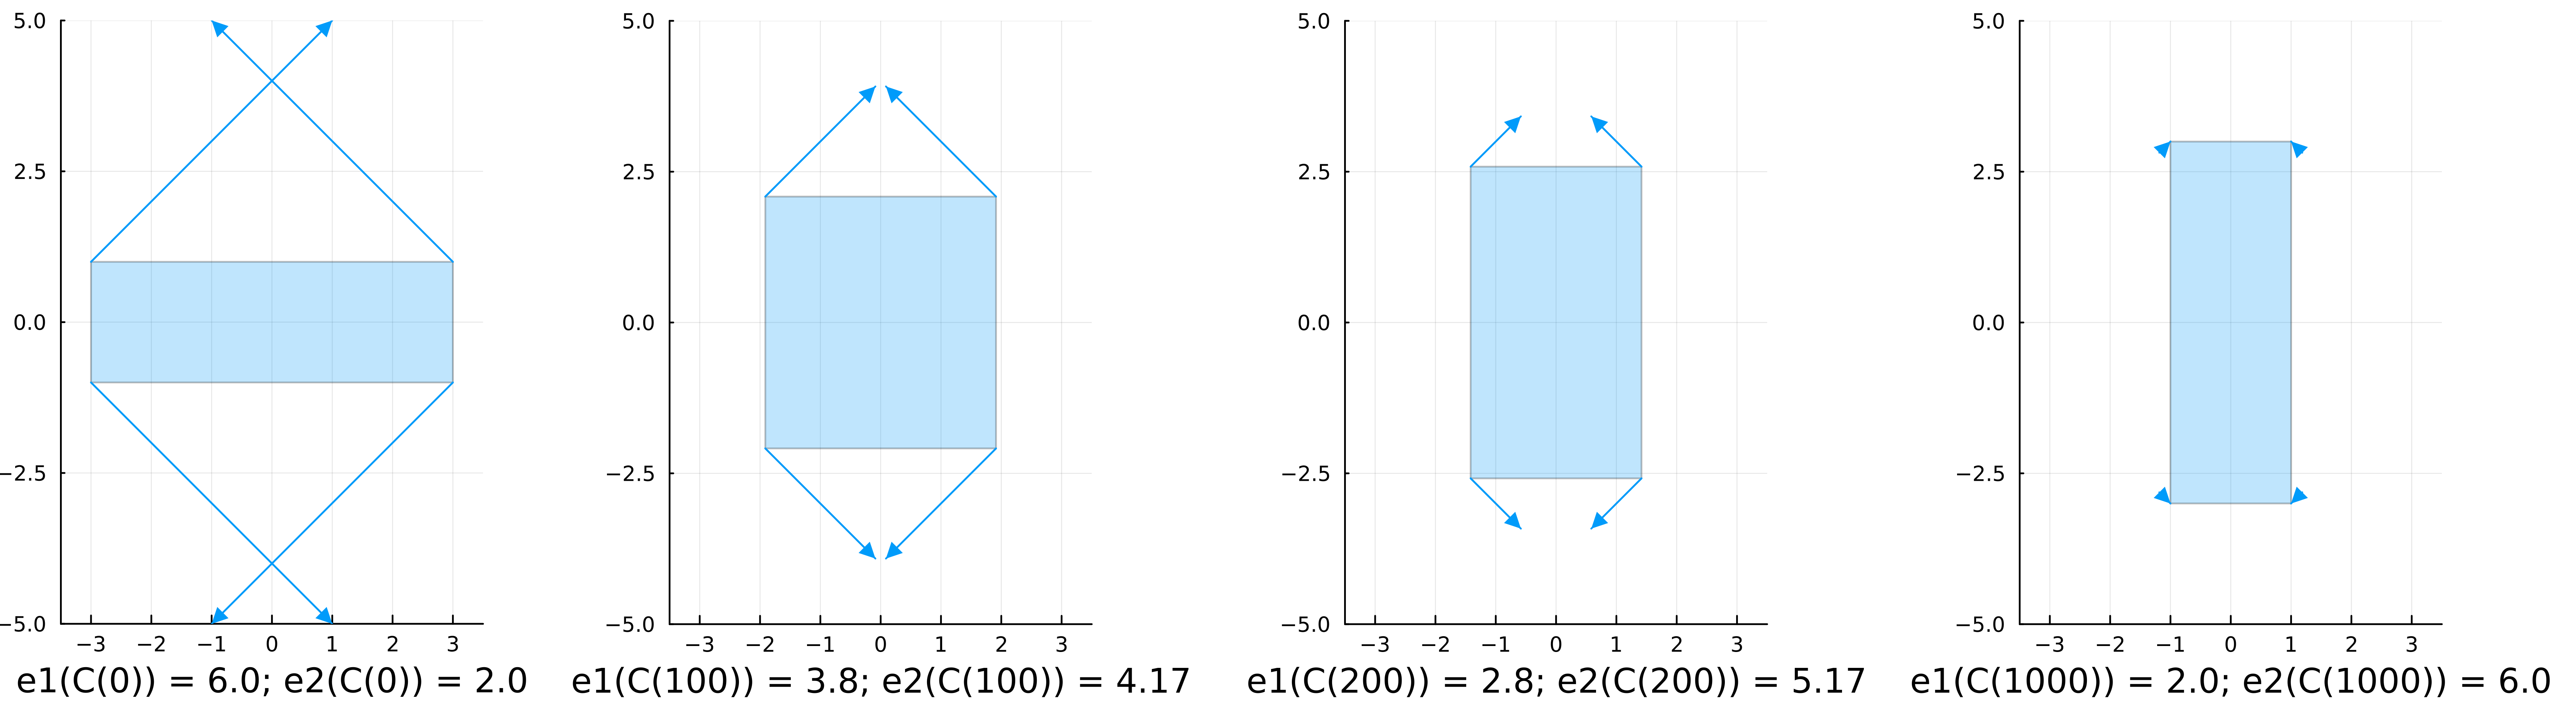
\includegraphics[width=15cm]{bachelors-thesis/forces/edge/edge1.png}
		\caption{The diagram illustrates the edge force acting on a DF cell.
		At time $t=0$, the cell is shaped as a rectangle $[-3,3]\times [-1,1]$, giving horizontal edges a length of 6 and vertical edges a length of 2.
		The corresponding edge lengths at the different time steps are annotated below each diagram.
		The target configuration is the rectangle $[-1,1]\times [-3,3]$, implying that the horizontal edges need to contract while the vertical edges must stretch.
		This transformation is clearly observable in the progression of the diagrams.
		}
		\label{fig:edgeForce}
	\end{center}
\end{figure}


\subsection{Interior angle force}
% mention scaling factor of /360 for interior angle force 
The combined application of the area and edge forces revealed instabilities in unfavorable configurations, where self-intersections of the cell edges occurred. 
Simulations without this energy sometimes can also result in constrictions at certain vertices, where the interior angle approaches $360$°. 
To address this issue, we introduce the interior angle energy. \\
The first challenge is to consistently determine the interior angle at a given vertex throughout the simulation.
Although we could apply the law of cosines and use $\arccos$ to compute the angle, this method would suffer from poor stability as the angle approaches $180$°.
A better alternative is to use the $\atanxy$ function, as it remains reliably stable at all angles. \\

\begin{definition} \textbf{arctan2} \\
	The function $$\atanxy:\R^2/\{0\} \rightarrow (-\pi, \pi]$$ is defined by:
	\begin{center}
		$ \atanxy(\vec{v}) = 
		\begin{cases}
			\arctan(\frac{v^{y}}{v^{x}}) & v^{x} > 0 \\
			\arctan(\frac{v^{y}}{v^{x}}) + \pi & v^{x} < 0, v^{y} > 0 \\
			\arctan(\frac{v^{y}}{v^{x}}) - \pi & v^{x} < 0, v^{y} < 0 \\
			\pi & v^{x} < 0, v^{y} = 0 \\
			\dfrac{\pi}{2} & v^{x} = 0, v^{y} > 0 \\ 		
			- \dfrac{\pi}{2} & v^{x} = 0, v^{y} < 0 \\ 
		\end{cases}. $
	\end{center}
\end{definition}

The $\atanxy(\vec{v})$ function computes the angle of a vector $\vec{v}$ with respect to the positive $x$ axis. \\
With this, we can compute the angles 
\begin{center}
	
	$\theta_1 = \atanxy( \vec{v}_{j-1} - \vec{v_j} )$, \\
	$\theta_2 = \atanxy( \vec{v}_{j+1} - \vec{v_j} )$
	
\end{center}
between the positive $x$ axis and the vectors from $\vec{v}_j$ to its neighboring vertices $\vec{v}_{j-1}$ and $\vec{v}_{j+1}$. 
We get the searched angle at $\vec{v}_j$ by subtracting $\theta_1 - \theta_2$.
To ensure that the angle lies within the interval $[0, 2\pi)$, we use the modulo operator $[ \cdot ]_{[0,2\pi)}$, which repeatedly adds or subtracts $2\pi$ from the angle until it falls within the desired range.
Thus, our interior angle operator is: 
\begin{center}
	$
	I^j_C = [\atanxy(\vec{v}_{j-1} - \vec{v_j}) - \atanxy(\vec{v}_{j+1} - \vec{v_j})]_{[0,2\pi)}.
	$
\end{center}

With that, we can define our interior angle energy. 
\begin{definition} \textbf{Interior angle energy} \\
	The energy $I: (\R^2)^{N_V} \rightarrow \R_{\geq 0}$ associated with preserving the cell interior angles is given by
	\begin{align}
		I_k(C) = \sum\limits_{j=1}^{N_V} \frac{1}{k}| I^j_{C} - I^{j}_d |^k, 
	\end{align}
	where $I^{j}_d$ is the desired interior angle at vertex $j$ and $I^j_{C}$ is the current interior angle at vertex $j$ of the considered cell. 
\end{definition}


We continue by computing the resulting force. 
The $\atanxy$ function is partly defined and not truly differentiable. 
We still want to compute a gradient to use it for our interior angle force. 
It is $$\atanxy(\vec{v}) = \arctan\left(\frac{v^{y}}{v^{x}} \right) + \text{constant}$$ almost everywhere, just not on areas with measure zero. 
We just compute the gradient of $\arctan(\frac{v^{y}}{v^{x}})$ instead. \\
Another problem is the modulo operator $[ \cdot ]_{[0,2\pi)}$, which is not differentiable at the interval limits.
However, we just neglect the modulo operator as it does not affect the dynamics of the gradient.

\begin{proposition} \textbf{Interior angle force} \\

	% The interior angle force $F^{(I)}_j(C): (\R^2)^{N_V} \rightarrow \R^2$ that gets applied on vertex $\vec{v}_j$ of cell $C$ is given by 
	% \begin{align}
	% 	\begin{split}
	% 		F^{(I)}_j(C) &= - \nabla_{\vec{v}_j} I(C)  \\
	% 			&= (I^{j-1}_d - I^{j-1}_{C}) \left( 
	% 				- \frac{1}{\norm[\vec{v}_{j} - \vec{v}_{j-1}]^{y}} \begin{pmatrix}
	% 					v_{j}^{y} - v_{j-1}^{y} \\[0.5em]
	% 					v_{j-1}^{x} - v_{j}^{x}
	% 				\end{pmatrix} 
	% 			\right) \\[0.5em] 
	% 		&+ (I^{j}_d - I^{j}_{C}) \left( 
	% 			\frac{1}{\norm[\vec{v}_{j-1} - \vec{v}_j]^{y}} \begin{pmatrix}
	% 			v_{j-1}^{y} - v_{j}^{y} \\[0.5em]
	% 			v_{j}^{x} - v_{j-1}^{x}
	% 			\end{pmatrix} 
	% 			- \frac{1}{\norm[\vec{v}_{j+1} - \vec{v}_j]^2} \begin{pmatrix}
	% 			v_{j+1}^{y} - v_{j}^{y} \\[0.5em]
	% 			v_{j}^{x} - v_{j+1}^{x}
	% 			\end{pmatrix} 
	% 			\right) \\[0.5em] 
	% 		&+ (I^{j+1}_d - I^{j+1}_{C}) \left( 
	% 			\frac{1}{\norm[\vec{v}_{j} - \vec{v}_{j+1}]^2} \begin{pmatrix}
	% 			v_{j}^{y} - v_{j+1}^{y} \\[0.5em]
	% 			v_{j+1}^{x} - v_{j}^{x}
	% 			\end{pmatrix} 
	% 			\right) %\\[0.5em] 
	% 	\end{split}
	% \end{align}

	The interior angle force $F_{k}^{(I)}: (\R^2)^{N_V} \rightarrow (\R^2)^{N_V}$ that gets applied on cell $C$ is given by  
	\begin{align*}
		F_{k}^{(I)}(C) 
		= - (\nabla_{\vec{v}_1} I_k(C), \ldots, \nabla_{\vec{v}_{N_V}} I_k(C))^T,
	\end{align*}
	where the gradient $\nabla_{\vec{v}_j} I_k(C)$ with respect to $\vec{v}_j = (v_{j}^{x}, v_{j}^{y})^T$ is given by 
	\begin{align}
		\begin{split}
			\nabla_{\vec{v}_j} I_k(C) &= \sgn(I^{j-1}_{C} - I^{j-1}_d) |I^{j-1}_{C} - I^{j-1}_d|^{k-1} \left( 
					- \frac{1}{\norm[\vec{v}_{j} - \vec{v}_{j-1}]^{y}} \begin{pmatrix}
						v_{j}^{y} - v_{j-1}^{y} \\[0.5em]
						v_{j-1}^{x} - v_{j}^{x}
					\end{pmatrix} 
				\right) \\[0.5em] 
			&+ \sgn(I^{j}_{C} - I^{j}_d)|I^{j}_{C} - I^{j}_d|^{k-1} \Biggl( 
				\frac{1}{\norm[\vec{v}_{j-1} - \vec{v}_j]^{y}} \begin{pmatrix}
				v_{j-1}^{y} - v_{j}^{y} \\[0.5em]
				v_{j}^{x} - v_{j-1}^{x}
				\end{pmatrix} \\
			&\hspace{1cm} - \frac{1}{\norm[\vec{v}_{j+1} - \vec{v}_j]^2} \begin{pmatrix}
				v_{j+1}^{y} - v_{j}^{y} \\[0.5em]
				v_{j}^{x} - v_{j+1}^{x}
				\end{pmatrix} 
				\Biggr) \\[0.5em] 
			&+ \sgn(I^{j+1}_{C} - I^{j+1}_d) |I^{j+1}_{C} - I^{j+1}_d|^{k-1} \left( 
				\frac{1}{\norm[\vec{v}_{j} - \vec{v}_{j+1}]^2} \begin{pmatrix}
				v_{j}^{y} - v_{j+1}^{y} \\[0.5em]
				v_{j+1}^{x} - v_{j}^{x}
				\end{pmatrix} 
				\right) %\\[0.5em] 
		\end{split}
		\label{gradient:angle}
	\end{align}
	for all $1 \leq j \leq N_V$.\\

	Proof. \\
	% TODO: check this force and the computations in the proof, especially the neighboring vertices part 
	We are looking for 
	\begin{center}
		$
		\nabla_{\vec{v}_j} I(C)
		$
	\end{center}
	
	Vertex $\vec{v}_j$ impacts the interior angles at $\vec{v}_{j-1}$, $\vec{v}_j$ and $\vec{v}_{j+1}$. 
	Thus, we get 
	\begin{align*}
		\nabla_{\vec{v}_j}  I_{k}(C) 
		&=  \nabla_{\vec{v}_j} \sum\limits_{j=1}^{N_V} \frac{1}{k}| I^j_{C} - I^{j}_d |^k \\
		&= \nabla_{\vec{v}_j} \frac{1}{k}| I^{j-1}_{C} - I^{j-1}_d |^k
		+ \nabla_{\vec{v}_j} \frac{1}{k}| I^{j}_{C} - I^{j}_d |^k
		+ \nabla_{\vec{v}_j} \frac{1}{k}| I^{j+1}_{C} - I^{j+1}_d |^k
	\end{align*}
	First, we will focus on the computation of $\nabla_{\vec{v}_j} \frac{1}{k}| I^{j}_{C} -  I^{j}_d |^k$. 

	\begin{align*}
		\nabla_{\vec{v}_j} \frac{1}{k}| I^{j}_{C} - I^{j}_d |^k 
		&= \sgn(I^j_{C} - I^{j}_d)|I^j_{C} - I^{j}_d|^{k-1} \nabla_{\vec{v}_j}  I^j_{C}   \\
		&= \sgn(I^j_{C} - I^{j}_d)|I^j_{C} - I^{j}_d|^{k-1} \cdot \\[0.2em]
		&\hspace{1cm} \nabla_{\vec{v}_j} [\atanxy(\vec{v}_{j-1} - \vec{v_j}) - \atanxy(\vec{v}_{j+1} - \vec{v_j})]_{[0,2\pi)}.
	\end{align*}
	At this point, the previously mentioned simplifications come into play and we use $\arctan \left(\frac{v_{j-1}^{y} - v_{j}^{y}}{v_{j-1}^{x} - v_{j}^{x}} \right)$ instead of $\atanxy(\vec{v}_{j-1} - \vec{v_j})$ and neglect the modulo operator. \\
	In the next step, we need to compute the gradient 
	\begin{center}
		$
		\nabla_{\vec{v}_j} \arctan \left(\dfrac{v_{j-1}^{y} - v_{j}^{y}}{v_{j-1}^{x} - v_{j}^{x}} \right).
		$
	\end{center}
	
	Therefore, we define helper functions 
	$$ f(\vec{v}) = \arctan\left( \frac{v^{y}}{v^{x}} \right)$$ 
	and 
	$$g(\vec{v}_{j-1}, \vec{v}_{j}) = \begin{pmatrix}
		v_{j-1}^{x} - v_{j}^{x} \\[0.5em] 
		v_{j-1}^{y} - v_{j}^{y}
	\end{pmatrix}.$$
	With these helper functions, we can write 
	$$ \arctan\left(\frac{v_{j-1}^{y} - v_{j}^{y}}{v_{j-1}^{x} - v_{j}^{x}}\right) = (f \circ g) (\vec{v}_{j-1}, \vec{v}_{j}) $$
	and use the two dimensional chain rule to stepwise compute the searched gradient. 
 
	\begin{center}
		
		$\dfrac{\partial f(\vec{v})}{\partial v^{x}} = \dfrac{1}{1 + \left(\dfrac{v^{y}}{v^{x}}\right)^2} \left(- \dfrac{v^{y}}{v^{x}}\right) = - \dfrac{v^{y}}{(v^{x})^2 + (v^{y})^2}$ \\
		$\dfrac{\partial f(\vec{v})}{\partial v^{y}} = \dfrac{1}{1 + \left(\dfrac{v^{y}}{v^{x}}\right)^2}  \dfrac{1}{v^{x}} =  \dfrac{v^{x}}{(v^{x})^2 + (v^{y})^2}$ \\ [0.5em]
		$ \nabla_{v_j^{x}} g(\vec{v}_{j-1}, \vec{v}_{j}) = (-1, 0)^T$ \\[0.3em]
		$ \nabla_{v_j^{y}} g(\vec{v}_{j-1}, \vec{v}_{j}) = (0, -1)^T$ 
	
	\end{center}

	With that, we can compute:
	\begin{align*}
		\frac{\partial (f \circ g) (\vec{v}_{j-1}, \vec{v}_j)}{\partial v_j^{x}} 
		&= ((\nabla f) \circ g (\vec{v}_{j-1}, \vec{v}_j))^T \cdot \nabla_{v_j^{x}} g (\vec{v}_{j-1}, \vec{v}_j) \\[0.5em]
		&= \begin{pmatrix}
			- \frac{v_{j-1}^{y} - v_{j}^{y}}{(v_{j-1}^{x} - v_{j}^{x})^2 + (v_{j-1}^{y} - v_{j}^{y})^2} \\[1.0em]
			\frac{v_{j-1}^{x} - v_{j}^{x}}{(v_{j-1}^{x} - v_{j}^{x})^2 + (v_{j-1}^{y} - v_{j}^{y})^2}
		\end{pmatrix}^T
		\cdot 
		\begin{pmatrix}
			-1 \\
			0
		\end{pmatrix} \\[0.5em]
		&= \frac{v_{j-1}^{y} - v_{j}^{y}}{(v_{j-1}^{x} - v_{j}^{x})^2 + (v_{j-1}^{y} - v_{j}^{y})^2} \\[0.5em]
		&= \frac{v_{j-1}^{y} - v_{j}^{y}}{\norm[\vec{v}_{j-1} - \vec{v}_j]^2}
	\end{align*}

	And similarly:
	\begin{align*}
		\frac{\partial (f \circ g) (\vec{v}_{j-1}, \vec{v}_j)}{\partial v_j^{y}} 
		&= ((\nabla f) \circ g (\vec{v}_{j-1}, \vec{v}_j))^T \cdot \nabla_{v_j^{y}} g (\vec{v}_{j-1}, \vec{v}_j) \\[0.5em]
		&= \begin{pmatrix}
			- \frac{v_{j-1}^{y} - v_{j}^{y}}{(v_{j-1}^{x} - v_{j}^{x})^2 + (v_{j-1}^{y} - v_{j}^{y})^2} \\[1.0em]
			\frac{v_{j-1}^{x} - v_{j}^{x}}{(v_{j-1}^{x} - v_{j}^{x})^2 + (v_{j-1}^{y} - v_{j}^{y})^2}
		\end{pmatrix}^T
		\cdot 
		\begin{pmatrix}
			0 \\
			-1
		\end{pmatrix} \\[0.5em]
		&= - \frac{v_{j-1}^{x} - v_{j}^{x}}{(v_{j-1}^{x} - v_{j}^{x})^2 + (v_{j-1}^{y} - v_{j}^{y})^2} \\[0.5em]
		&= \frac{v_{j}^{x} - v_{j-1}^{x}}{\norm[\vec{v}_{j-1} - \vec{v}_j]^2} \\[0.5em]
	\end{align*}

	Overall, we get 
	\begin{align*}
		\nabla_{\vec{v}_j} \arctan \left(\frac{v_{j-1}^{y} - v_{j}^{y}}{v_{j-1}^{x} - v_{j}^{x}} \right) = \frac{1}{\norm[\vec{v}_{j-1} - \vec{v}_j]^2} \begin{pmatrix}
			v_{j-1}^{y} - v_{j}^{y} \\[0.5em]
			v_{j}^{x} - v_{j-1}^{x}
		\end{pmatrix}.
	\end{align*}
	
	Thus, we can come back to: 
	\begin{align*}
		\nabla_{\vec{v}_j} \frac{1}{k}| I^{j}_{C} - I^{j}_d |^k 
		&= \sgn(I^j_{C} - I^{j}_d)|I^j_{C} - I^{j}_d|^{k-1} \nabla_{\vec{v}_j} I^j_{C} \\
		&= \sgn(I^j_{C} - I^{j}_d)|I^j_{C} - I^{j}_d|^{k-1} \cdot \\
		&\hspace{1cm}  \Biggl( \arctan\left(\frac{v_{j-1}^{y} - v_{j}^{y}}{v_{j-1}^{x} - v_{j}^{x}}\right) - \arctan\left(\frac{v_{j+1}^{y} - v_{j}^{y}}{v_{j+1}^{x} - v_{j}^{x}}\right)\Biggr) \\
		&= \sgn(I^j_{C} - I^{j}_d)|I^j_{C} - I^{j}_d|^{k-1} \cdot \\
		& \hspace{1cm} \Biggl( \frac{1}{\norm[\vec{v}_{j-1} - \vec{v}_j]^2} \begin{pmatrix}
			v_{j-1}^{y} - v_{j}^{y} \\[0.5em]
			v_{j}^{x} - v_{j-1}^{x}
		\end{pmatrix} - \frac{1}{\norm[\vec{v}_{j+1} - \vec{v}_j]^2} \begin{pmatrix}
			v_{j+1}^{y} - v_{j}^{y} \\[0.5em]
			v_{j}^{x} - v_{j+1}^{x}
		\end{pmatrix} \Biggr).
	\end{align*}

	For the neighboring vertices, we need:
	\begin{gather*}
		\nabla_{\vec{v}_j} \arctan\left( \frac{v_j^y - v_{j-1}^y}{v_j^x - v_{j-1}^x} \right) \text{ and  } \; \nabla_{\vec{v}_j} \arctan\left( \frac{v_j^y - v_{j+1}^y}{v_j^x - v_{j+1}^x} \right).
	\end{gather*}
	Therefore, we can use the same helper function \[f(\vec{v}) = \arctan\left( \frac{v^{y}}{v^{x}} \right),\]
	but we need different functions for $g$, as the arrangement of the vertex coordinates differs a bit. 
	We introduce \[g_{-}(\vec{v}_{j-1}, \vec{v}_{j}) = \begin{pmatrix}
		v_{j}^{x} - v_{j-1}^{x} \\[0.5em] 
		v_{j}^{y} - v_{j-1}^{y}
	\end{pmatrix} = - g(\vec{v}_{j-1}, \vec{v}_{j}).\] 
	and
	\[g_{+}(\vec{v}_{j}, \vec{v}_{j+1}) = \begin{pmatrix}
		v_{j}^{x} - v_{j+1}^{x} \\[0.5em] 
		v_{j}^{y} - v_{j+1}^{y}
	\end{pmatrix}.
	\] 
	The gradients are 
	\[
		\nabla_{v_j^x} g_{-}(\vec{v}_{j-1}, \vec{v}_{j}) = (1,0)^T, \nabla_{v_j^y} g_{-}(\vec{v}_{j-1}, \vec{v}_{j}) = (0,1)^T,
	\]
	\[
	\nabla_{v_j^x} g_{+}(\vec{v}_{j-1}, \vec{v}_{j}) = (1,0)^T, \nabla_{v_j^y} g_{+}(\vec{v}_{j-1}, \vec{v}_{j}) = (0,1)^T.
	\]
	Thus, the Jacobian of both $g_{-}$ and $g_{+}$ is the identity matrix and we can just neglect it in the following chain rules. 
	For the previous vertex, we get 
	\begin{align*}
		\nabla_{\vec{v}_j} \frac{1}{k}| I^{j+1}_{C} - I^{j+1}_d |^k 
		&= \sgn(I^{j-1}_{C} - I^{j-1}_d)|I^{j-1}_{C} - I^{j-1}_d|^{k-1} \cdot \\[0.5em]
		&\hspace{1cm} \nabla_{\vec{v}_j} \left(\arctan\left(\frac{v_{j-2}^{y} - v_{j-1}^{y}}{v_{j-2}^{x} - v_{j-1}^{x}}\right) - \arctan\left(\frac{v_{j}^{y} - v_{j-1}^{y}}{v_{j}^{x} - v_{j-1}^{x}}\right)\right) \\[0.5em]
		&= \sgn(I^{j-1}_{C} - I^{j-1}_d)|I^{j-1}_{C} - I^{j-1}_d|^{k-1} \cdot \\
		&\hspace{1cm} \nabla_{\vec{v}_j} \left(- \arctan\left(\frac{v_{j}^{y} - v_{j-1}^{y}}{v_{j}^{x} - v_{j-1}^{x}}\right)\right) \\[0.5em]
		&= \sgn(I^{j-1}_{C} - I^{j-1}_d)|I^{j-1}_{C} - I^{j-1}_d|^{k-1} \cdot \\
		&\hspace{1cm} - \nabla_{\vec{v}_j} \left( f \circ g_{-}(\vec{v}_{j-1}, \vec{v}_{j-1}) \right) \\[0.5em]
		&= \sgn(I^{j-1}_{C} - I^{j-1}_d)|I^{j-1}_{C} - I^{j-1}_d|^{k-1} \cdot \\
		&\hspace{1cm} - (\nabla f) \circ g_{-}(\vec{v}_{j-1}, \vec{v}_{j-1}) \\[0.5em]
		&= \sgn(I^{j-1}_{C} - I^{j-1}_d)|I^{j-1}_{C} - I^{j-1}_d|^{k-1} \cdot \\
		&\hspace{1cm} - \frac{1}{\norm[\vec{v}_j - \vec{v}_{j-1}]^2} (v_j^y - v_{j-1}^y, v_{j-1}^x - v_j^x)^T.		
	\end{align*}
	Finally, for the successor vertex, we get 
	\begin{align*}
		\nabla_{\vec{v}_j} \frac{1}{k}| I^{j+1}_{C} - I^{j+1}_d |^k 
		&= \sgn(I^{j+1}_{C} - I^{j+1}_d)|I^{j+1}_{C} - I^{j+1}_d|^{k-1} \cdot \\[0.5em]
		&\hspace{1cm} \nabla_{\vec{v}_j} \left(\arctan\left(\frac{v_{j}^{y} - v_{j+1}^{y}}{v_{j}^{x} - v_{j+1}^{x}}\right) - \arctan\left(\frac{v_{j+2}^{y} - v_{j+1}^{y}}{v_{j+2}^{x} - v_{j+1}^{x}}\right)\right) \\[0.5em]
		&= \sgn(I^{j+1}_{C} - I^{j+1}_d)|I^{j+1}_{C} - I^{j+1}_d|^{k-1} \cdot \\
		&\hspace{1cm} \nabla_{\vec{v}_j} \left(\arctan\left(\frac{v_{j}^{y} - v_{j+1}^{y}}{v_{j}^{x} - v_{j+1}^{x}}\right)\right) \\[0.5em]
		&= \sgn(I^{j+1}_{C} - I^{j+1}_d)|I^{j+1}_{C} - I^{j+1}_d|^{k-1} \cdot \\
		&\hspace{1cm} \nabla_{\vec{v}_j} \left( f \circ g_{+}(\vec{v}_{j-1}, \vec{v}_{j-1}) \right) \\[0.5em]
		&= \sgn(I^{j+1}_{C} - I^{j+1}_d)|I^{j+1}_{C} - I^{j+1}_d|^{k-1} \cdot \\
		&\hspace{1cm} (\nabla f) \circ g_{+}(\vec{v}_{j-1}, \vec{v}_{j-1}) \\[0.5em]
		&= \sgn(I^{j+1}_{C} - I^{j+1}_d)|I^{j+1}_{C} - I^{j+1}_d|^{k-1} \cdot \\
		&\hspace{1cm} - \frac{1}{\norm[\vec{v}_j - \vec{v}_{j+1}]^2} (v_j^y - v_{j+1}^y, v_{j+1}^x - v_j^x)^T.	
	\end{align*}
	\qed
\end{proposition}

Figure \ref{fig:angleForce} illustrates the isolated effect of the interior angle force.

\begin{figure}
	\begin{center}
		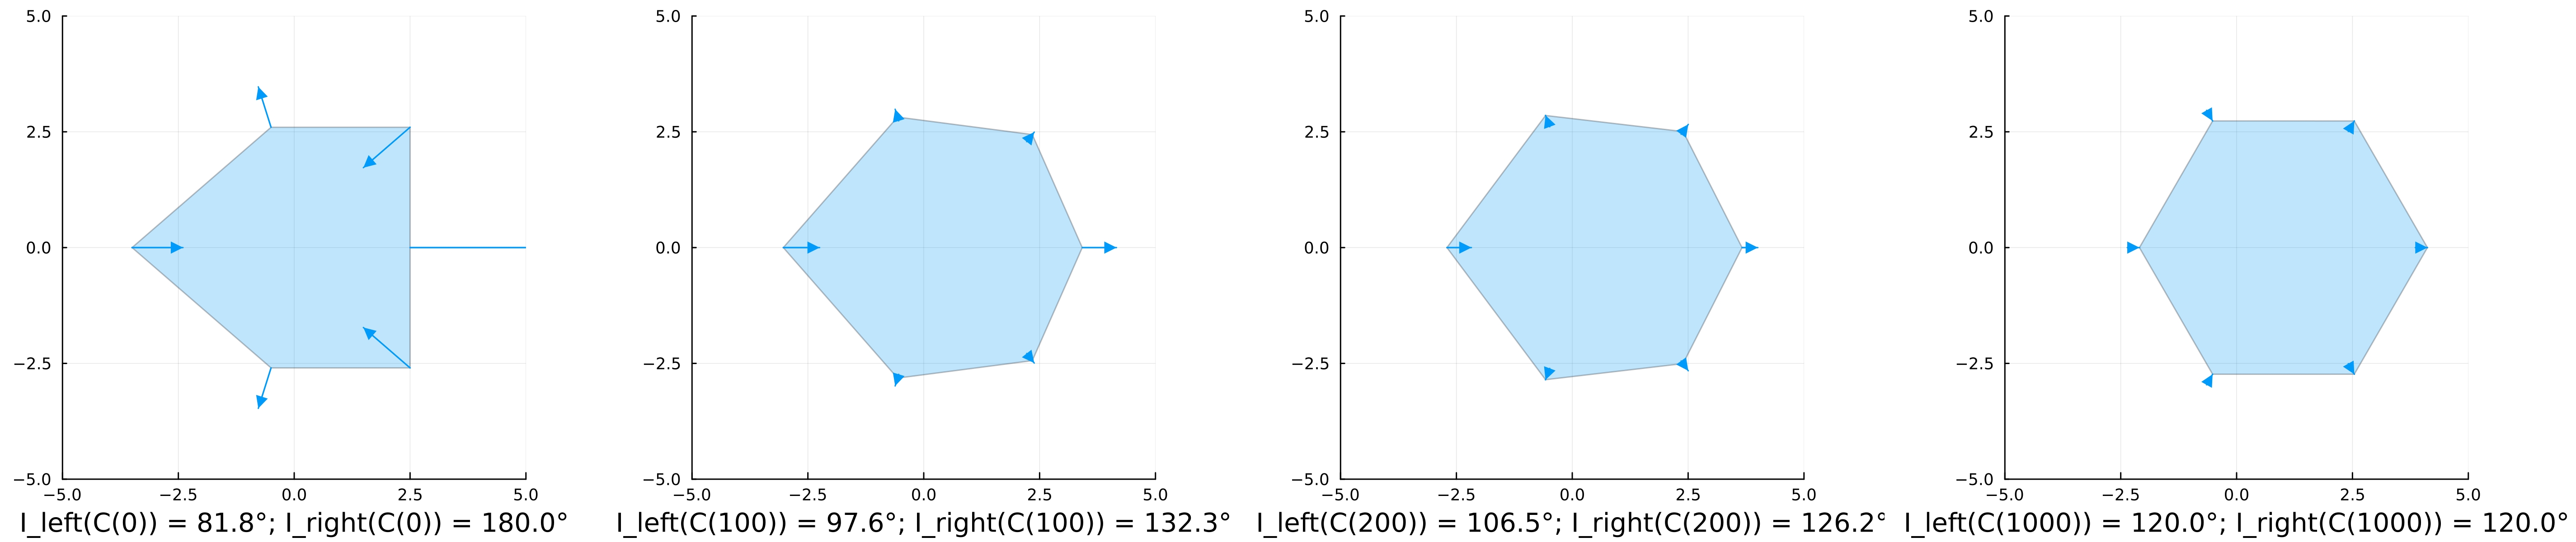
\includegraphics[width=15cm]{bachelors-thesis/forces/angle/angle1.png}
		\caption{The figure illustrates the action of the interior angle force on the vertices of a DF cell.
		The initial state, shown in the first plot, must be mirrored horizontally to achieve the desired state depicted in the final plot.
		This reshaping shows on the one hand that the dynamic is capable of decreasing interior angles from $270$° to $90$° and on the other hand it can also increase interior angles from $90$° to $270$°. 
		Below each chart, we can see the current interior angles of the two vertices that have the $y$ value zero. 
		}
		\label{fig:angleForce}
	\end{center}
\end{figure}





 

\subsection{Overlap force}
% explain the algorithm
Unlike the previous energies, which act independently on each cell, the overlap force is the first to account for interactions between multiple cells, thereby introducing cell-to-cell interaction into the simulation. \\
The challenging aspect of computing the overlap force lies in detecting overlaps within the cell system. 
An overlap is treated as a DF cell in its own right, composed of the vertices from each of the two overlapping cells that lie inside the other, along with the two intersection points where the cell boundaries intersect. \\ 
Once all overlaps have been identified, we apply a dynamic similar to that of the area force, but with a desired area of zero. 
This generates a force that acts to eliminate the overlap by reducing its area to zero. 
The resulting force is then applied to the vertices of the original cells that define the overlapping region. \\
The first step in detecting overlaps is identifying the intersection points between cell boundaries.
Intersections can be identified by representing the cell edges as line segments and computing the intersection points between segments belonging to different cells. \\
Having found all intersections, we can apply the following algorithm, that can be used to compute all overlaps between two cells. 

\begin{algorithm} \textbf{Computation of a discrete overlap} \label{alge:discreteOverlap}
	\begin{itemize} 
		\itemsep0em 
		\item[] \text{INPUT:}
		\item Discrete cells  $C$and $\zeta$
		\item List $I$ of unused intersections of $C$ and $\zeta$ 
	\end{itemize}
	\begin{algorithmic}
		\Function{constructOverlap}{$C$, $\zeta$, $I$}		
			\State usedIntersections = List$\{$Intersection$\}$(I[1]) 
			\State newOverlap = List$\{$Vertices$\}$(I[1]) 
			\State currentIntersection = I[1]
			
			\For{counter = 1 : length(I)} 
			
				\If{counter is even}
					\State newPath, newIntersection = findPath(currentIntersection, $C$, $I$) 
				\Else 
					\State newPath, newIntersection = findPath(currentIntersection, $\zeta$, $I$) 
				\EndIf
				
				\State append!(newOverlap, newPath)
				\If{newIntersection == I[1]} 
					\State \Return newOverlap, usedIntersections
				\Else 
					\State append!(newOverlap, newIntersection)
					\State append!(usedIntersections, newIntersection) 
					\State currentIntersection = newIntersection
				\EndIf
			\EndFor
		\EndFunction
	\end{algorithmic}
	\begin{itemize} 
		\itemsep0em 
		\item[] \text{OUTPUT:}
		\item A single intersection `newOverlap' which occurs between $C$ and $\zeta$ and which uses vertices from  $C$ and $\zeta$ as well as only intersections from $I$
		\item A list `usedIntersections' of all intersection that are used in `newOverlap'
	\end{itemize}	
\end{algorithm}
%TODO; rewrite that shit 
The algorithm begins by selecting the first intersection point $I[1]$ from the list $I$ as the initial vertex of the overlap cell `newOverlap'. 
This point is also added to the list `usedIntersections' \\
Next, the function `getOverlap' calls another function, `findPath', which determines the path along the discrete cell $\zeta$ from the current intersection point to the next intersection in $I$ encountered while traversing the edges of $\zeta$. 
This next intersection is also returned by the function. 
The identified path is a list of vertices in $\zeta$ that lie strictly between the two intersections. 
It may be empty if the next intersection occurs on the same edge as the current one. 
Both the path and the newly found intersection are appended to `newOverlap', and the intersection is also added to the list usedIntersections.\\
Since each intersection implies changing the cell from which the overlapping cell uses the edges, `findPath' is now applied to the other cell. 
Again, it will deliver the next intersection as well as a list of the in between laying vertices. 
The vertex list always gets appended to `newOverlap'. \\
If the newly found intersection is equal to the initial intersection $I[1]$, then the construction of the discrete overlap cell `newOverlap' is complete. 
At this point, both `newOverlap' and `usedIntersections' can be returned by the function `constructOverlap'. \\
Otherwise, the newly found intersection is appended to both `newOverlap' and `usedIntersections', and the process continues by calling `findPath' on the other discrete cell.   
This step is repeated until the starting intersection is reached, completing the overlap cell construction. \\
Once an overlap between $C$ and $\zeta$ has been successfully extracted, all intersections used in its construction can be removed from the list $I$, since each intersection point belongs to exactly one overlap. 
As long as $I$ is not empty, the function `constructOverlap' can be called again with the updated list to extract the next overlap. 
When $I$ is empty, we can be certain that all intersections between $C$ and $\zeta$ have been processed, and thus all overlaps between the two cells have been identified. \\

Each time `findPath' is called, it is not immediately clear in which direction the function should traverse the vertices of the given cell. 
However, the correct direction can be determined using the following approach. \\
Starting from the current intersection passed into the function, move a small distance in one direction along the edge of the given cell where the intersection is located. Next, check whether this new point lies within the boundaries of the other cell as well. 
If the point is found in both cells, the chosen direction is correct. 
If not, then the opposite direction must be used. \\ 
A simple method to determine whether a point lies inside a polygon is to draw a ray from the point to the outside of the polygon. 
The number of intersections between the ray and the polygon's edges determines the point's position. 
If the number of intersections is odd, the point is inside the polygon.
If it is even, the point is outside the polygon. \\ 
\smallskip  \\
% until here the rewriting!! 
% then continue with the energy and the force 
After introducing the method for detecting overlaps, we can now define the overlap force, which acts on the cell vertices involved in an overlap. 
This force is first computed based on the geometry of the overlap and then distributed to the corresponding vertices of the original cells. 

\begin{definition} \textbf{Overlap energy} \\
	Let $C_i$ and $C_k$ be two cells from the system $\vec{C}$ and $\Omega_{i,k}$ be the set of all overlaps that appear between $C_i$ and $C_k$, like explained above. Then, the total overlap energy of the cell system is given by the formula 
	\begin{align}
		O_k(C, \vec{C}) = \sum\limits_{i=1}^{N_C} \left( \sum\limits_{m=i+1}^{N_C} \left(\sum\limits_{D_l \in \Omega_{i,m}} \frac{1}{k}|A_{D_l}|^k\right) \right),		
	\end{align} 
	where $A_{D_l}$ is the area of the overlap $D_l$.  \\
\end{definition}

To decrease the overlap areas during the simulation, we evaluate the gradient flow of the area energy with a desired area of zero which indicates the direction of motion for each vertex for reducing the overlap areas.

\begin{proposition} \textbf{Overlap force} \\
	The overlap force $F_{k}^{(O)}: (\R^2)^{N_V} \times (\R^2)^{N_V N_C} \rightarrow (\R^2)^{N_V}$ that gets applied on cell $C = (\vec{v}_1, \ldots, \vec{v}_{N_V})$ is given by  
	\begin{align*}
		F_{k}^{(O)}(C, \vec{C}) 
		= - (\nabla_{\vec{v}_1} O_k(C, \vec{C}), \ldots, \nabla_{\vec{v}_{N_V}} O_k(C, \vec{C}))^T,
	\end{align*}
	where the gradient $\nabla_{\vec{v}_j} O_k(C, \vec{C})$ with respect to $\vec{v}_j = (v_{j}^{x}, v_{j}^{y})^T$ is given by 
	\begin{align}
		\begin{split}
			\nabla_{\vec{v}_j} O_k(C, \vec{C}) &= \sum\limits_{m=1, m \neq i}^{N_C} \left( \sum\limits_{D_l \in \Omega_{i,m}} \delta_{\vec{v}_j}(D_l)  \dfrac{1}{2} |A_{D_l}|^{k-1} \begin{pmatrix} d_{j+1}^{D_l, 2} - d_{j-1}^{D_l, 2} \\[0.5em]  d_{j-1}^{D_l, 1} - d_{j+1}^{D_l, 1} \end{pmatrix} \right)
		\end{split}
		\label{gradient:overlap}
	\end{align}
	for all $1 \leq j \leq N_V$, where $\Omega_{i,k}$ is the set of all overlaps that arise between the cells $i$ and $k$, $\vec{d}_{j-1}^{\: D_l} = (d_{j-1}^{D_l, 1}, d_{j-1}^{D_l, 2})^T$ and $\vec{d}_{j+1}^{\: D_l} = (d_{j+1}^{D_l, 1}, d_{j+1}^{D_l, 2})^T$ are the neighboring vertices of $\vec{v}_j$ in the overlap $D_l$ and $A_{D_l}$ is the area of the overlap $D_l$.\\
	The dirac $\delta_{\vec{v}_j}(D_l)$ equals one, if $\vec{v}_j$ is a vertex of the overlap $D_l$ and zero otherwise. \\

	Proof. \\
	
	Let us begin with the computation:
	\begin{align*}
		\nabla_{\vec{v}_j} \frac{1}{k}|A_{D_l}|^k
		&= \begin{cases}
			\nabla_{\vec{v}_j} \frac{1}{k} |A_{D_l}|^k &\text{ if } \vec{v}_j \in D_l \\
			0 &\text{ if } \vec{v}_j \notin D_l
		\end{cases} \\
		&= \delta_{\vec{v}_j}(D_l)  \nabla_{\vec{v}_j} \frac{1}{k}|A_{D_l} - 0|^k \\
		&= \delta_{\vec{v}_j}(D_l)  \nabla_{\vec{v}_j} A_k(D_l) \\
		&= \delta_{\vec{v}_j}(D_l)  \dfrac{1}{2} \sgn(A_{D_l} - 0) |A_{D_l} - 0|^{k-1} 
		\begin{pmatrix} d_{j+1}^{D_l, 2} - d_{j-1}^{D_l, 2} \\[0.5em]  d_{j-1}^{D_l, 1} - d_{j+1}^{D_l, 1} \end{pmatrix} \\
		&= \delta_{\vec{v}_j}(D_l)  \dfrac{1}{2} |A_{D_l}|^{k-1} 
		\begin{pmatrix} d_{j+1}^{D_l, 2} - d_{j-1}^{D_l, 2} \\[0.5em]  d_{j-1}^{D_l, 1} - d_{j+1}^{D_l, 1} \end{pmatrix}, \\
	\end{align*}
	where we obeserved the presence of the area energy $A_k(D_l) = \frac{1}{k}|A_{D_l} - 0|^k$ and used the area gradient from Formula \ref{gradient:area}. 
	The desired cell area of the overlap is always zero, as we want to achieve a setting without overlaps. 
	The vertices $\vec{d}_{j-1}^{\: D_l}$ and $\vec{d}_{j+1}^{\: D_l}$ represent the neighboring vertices of $\vec{v}_j$ in the overlap cell. \\
	Overall, we get:
	\begin{align*}
		\nabla_{\vec{v}_j^{\: i}} O_k(C_i, \vec{C}) 
		&= \nabla_{\vec{v}_j^{\: i}} \sum\limits_{n=1}^{N_C} \left( \sum\limits_{m=n+1}^{N_C}  \left(\sum\limits_{D_l \in \Omega_{n,m}} \frac{1}{k}|A_{D_l}|^k\right) \right) \\
		&= \nabla_{\vec{v}_j^{\: i}} \sum\limits_{m=1, m \neq i}^{N_C} \left( \sum\limits_{D_l \in \Omega_{i,m}} \frac{1}{k}|A_{D_l}|^k\right)\\
		&= \sum\limits_{m=1, m \neq i}^{N_C} \left( \sum\limits_{D_l \in \Omega_{i,m}} \nabla_{\vec{v}_j^{\: i}} \frac{1}{k}|A_{D_l}|^k\right)\\
		&= \sum\limits_{m=1, m \neq i}^{N_C} \left( \sum\limits_{D_l \in \Omega_{i,m}} \delta_{\vec{v}_j^{\: i}}(D_l)  \dfrac{1}{2} |A_{D_l}|^{k-1} 
		\begin{pmatrix} d_{j+1}^{D_l, 2} - d_{j-1}^{D_l, 2} \\[0.5em]  d_{j-1}^{D_l, 1} - d_{j+1}^{D_l, 1} \end{pmatrix}\right)\\
	\end{align*}

	\qed
\end{proposition}

Figure \ref{fig:overlapForce} illustrates the interaction between two overlapping cells, highlighting the effect of the overlap force on their vertices.
\begin{figure}[h!]
	\begin{center}
		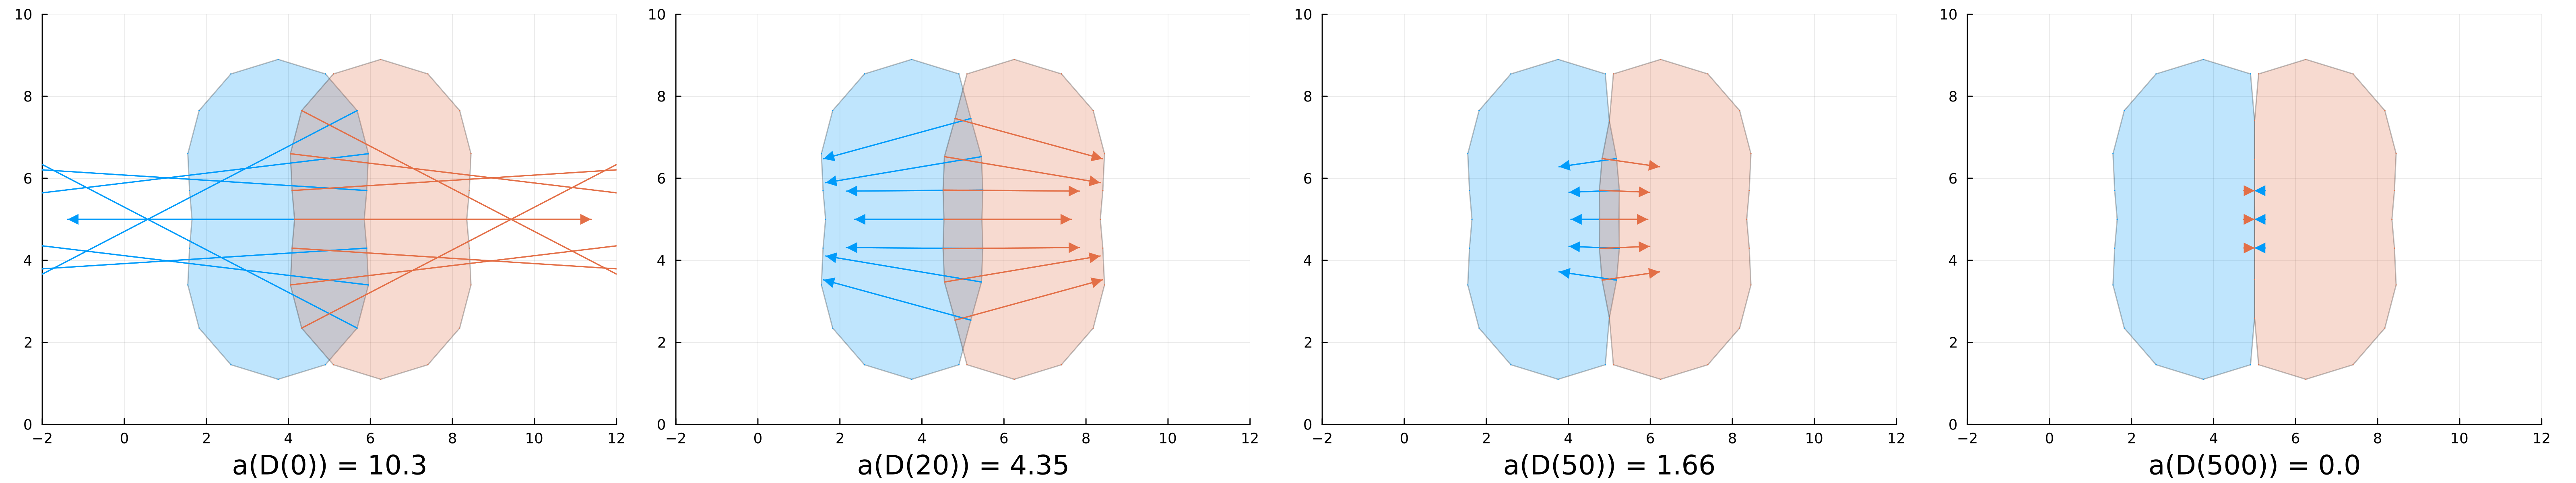
\includegraphics[width=15cm]{bachelors-thesis/forces/overlap/overlap1.png}
			\caption{This figure demonstrates how the overlap force acts on two overlapping DF cells.
			The blue arrows indicate the forces acting on the blue cell, while the red arrows represent those acting on the red cell.
			The current overlap areas at each time step are displayed below the corresponding diagrams.			
			On each consecutive diagram, we can see that the overlap gets reduced, until the area of the overlap is zero.  }
			\label{fig:overlapForce}
	\end{center}
\end{figure}


\subsection{A simulation run}
% state the force system
% DifferentialEquations.jl solver \\
%  -> Euler Maruyama method with fixed time step size  \\